\newpage

\begin{usecase}
    \addheading{Use-Case Description}
    \addsingletwocolumnrow{Name}{oeReportOnCrisis}
    \addsingletwocolumnrow{Scope}{System}
    \addsingletwocolumnrow{Altitude}{subfunction}
    \addrowheading{Parameters}
    \addnumberedsinglerow{}{\msrcode{AlertID:dtAlertID} - the identification of the Alert.}
    \addnumberedsinglerow{}{\msrcode{AText:dtComment} - a text written by the \msr{actCoordinator} to better describe the crisis, in his own words, in the report.}
    \addnumberedsinglerow{}{\msrcode{UserID:dtUserID} - a unique identifier identifying the \msrcode{actCoordinator} writing the report.}
    \addnumberedsinglerow{}{\msrcode{TypeofCrisis:etCrisisType} - the type of the crisis differentiated here by (Small, Medium or Huge) thus describing the crisis type.}
    \addnumberedsinglerow{}{\msrcode{CrisisStatus:etCrisisStatus} - the status of the crisis differentiated here by (pending, handled or solved).}
    \addnumberedsinglerow{}{\msrcode{RecievedMessages:dtRecievedMessage} - This is a record of the alert messages received from the actor \msrcode{actComCompany}.}
    \addnumberedsinglerow{}{\msrcode{NumberofVehiculesinaccident:dtNbrofVehiculesInAccident} - the number of vehicles involved in the accident.}
    \addnumberedsinglerow{}{\msrcode{NumberofVictimsinaccident:dtNbrofVictims} - the number of victims involved in the accident.}
    \addrowheading{Primary actor(s)}
    \addnumberedsinglerow{}{\msrcode{Coordinator[active]}}
    \addrowheading{Secondary actor(s)}
    \addnumberedsinglerow{}{\msrcode{ComCompany[passive]}}
    \addrowheading{Goal(s) description}
    \addsinglerow{the \msrcode{actCoordinator}'s goal is to write a report about the current ongoing crisis or to write a final report of the crisis.}
    \addrowheading{Reuse}
    \addnumberedsinglerow{}{none}
    \addrowheading{Protocol condition(s)}
    \addnumberedsinglerow{}{the \msricrash system has been deployed.}
    \addnumberedsinglerow{}{an Alert has been received by our system.}
    \addnumberedsinglerow{}{the \msrcode{actDomainExpert} has validated the alert.}
    \addnumberedsinglerow{}{the \msrcode{actCoordinator} actor has the right domain to access the Crisis and is thus allowed to write a report about it.}
    \addrowheading{Pre-condition(s)}
    \addnumberedsinglerow{}{none}
    \addrowheading{Main post-condition(s)}
    \addnumberedsinglerow{}{A report of a certain crisis exists in the system.}
    \addrowheading{Main success steps}
    \addalphanumberedsinglerow{}{the actor \msrcode{actCoodinator} sends the message\msrcode {oeReportOnCrisis(dtAlertID AdtCrisisID, dtComment AdtComment, dtUserID AdtUserID, etCrisisType AdtCrisisType, etCrisisStatus AdtCrisisStatus, dtRecievedMessage AdtReceivedMessage, dtNbrofVehiculesInAccident AdtVehiculesInAccident, dtNbrOfVictims AdtNbrVictims)} to the system.}
    \addrowheading{Step Constraints Ordering and Extensions}
    \addnumberedsinglerow{}{none}
    \addrowheading{Additional Information}
    \addsinglerow{The coordinator decided ultimately what information is put into the report the shown data types are only meant as an example of what can be added to such a report.}
\end{usecase}

\clearpage

\begin{figure}[htbp]
\begin{center}
\scalebox{0.95}{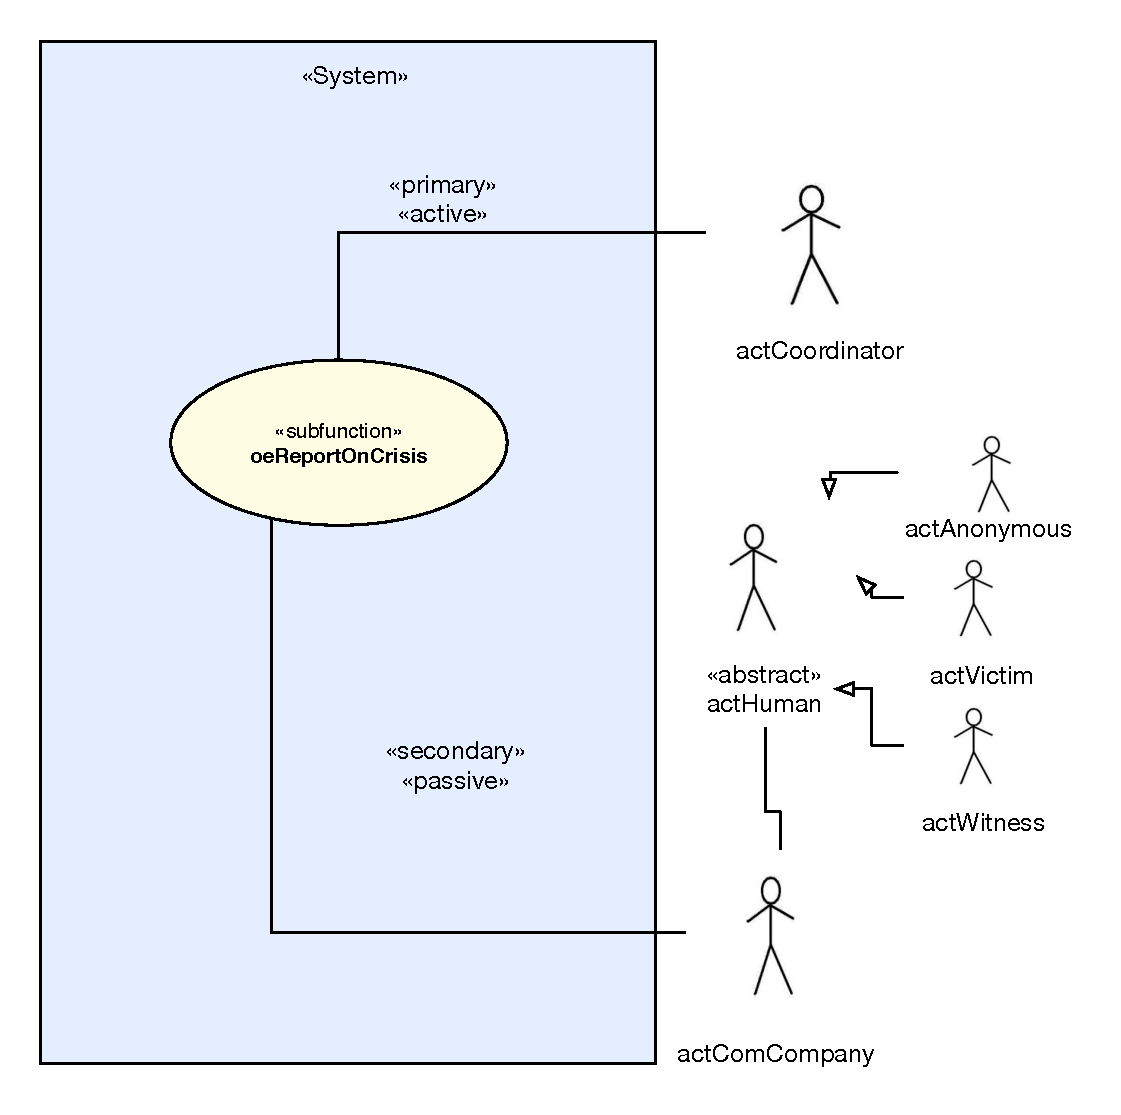
\includegraphics[width=180mm]{./images/oeReportOnCrisis.eps}\normalsize}
\end{center}
\caption[\msricrash Use Case Diagram: oeReportOnCrisis Diagram]{\msricrash Use Case Diagram: oeReportOnCrisis}
\label{fig:icrash-RE-UCD-oeReportOnCrisis}
\end{figure}
\vspace{0.5cm}

